% !TEX TS-program = pdflatex
% !TEX encoding = UTF-8 Unicode

% This is a simple template for a LaTeX document using the "article" class.
% See "book", "report", "letter" for other types of document.

\documentclass[11pt,fleqn]{article} % use larger type; default would be 10pt

\usepackage[utf8]{inputenc} % set input encoding (not needed with XeLaTeX)

%%% Examples of Article customizations
% These packages are optional, depending whether you want the features they provide.
% See the LaTeX Companion or other references for full information.

%%% PAGE DIMENSIONS
\usepackage{geometry} % to change the page dimensions
\geometry{letterpaper} % or letterpaper (US) or a5paper or....
% \geometry{margin=2in} % for example, change the margins to 2 inches all round
% \geometry{landscape} % set up the page for landscape
%   read geometry.pdf for detailed page layout information
\usepackage{upgreek}
\usepackage{graphicx} % support the \includegraphics command and options
\usepackage{subcaption}

% \usepackage[parfill]{parskip} % Activate to begin paragraphs with an empty line rather than an indent

%%% PACKAGES
\usepackage{booktabs} % for much better looking tables
%\usepackage{breqn}
\usepackage{amsmath}
\usepackage{array} % for better arrays (eg matrices) in maths
\usepackage{paralist} % very flexible & customisable lists (eg. enumerate/itemize, etc.)
\usepackage{verbatim} % adds environment for commenting out blocks of text & for better verbatim
%\usepackage{subfig} % make it possible to include more than one captioned figure/table in a single float
% These packages are all incorporated in the memoir class to one degree or another...
\setlength{\mathindent}{0pt}

%%% HEADERS & FOOTERS
\usepackage{fancyhdr} % This should be set AFTER setting up the page geometry
\pagestyle{fancy} % options: empty , plain , fancy
\renewcommand{\headrulewidth}{0pt} % customise the layout...
\lhead{}\chead{}\rhead{}
\lfoot{}\cfoot{\thepage}\rfoot{}

%%% SECTION TITLE APPEARANCE
\usepackage{sectsty}
\allsectionsfont{\sffamily\mdseries\upshape} % (See the fntguide.pdf for font help)
% (This matches ConTeXt defaults)

%%% ToC (table of contents) APPEARANCE
\usepackage[nottoc,notlof,notlot]{tocbibind} % Put the bibliography in the ToC
\usepackage[titles,subfigure]{tocloft} % Alter the style of the Table of Contents
\renewcommand{\cftsecfont}{\rmfamily\mdseries\upshape}
\renewcommand{\cftsecpagefont}{\rmfamily\mdseries\upshape} % No bold!

%%% END Article customizations

%%% The "real" document content comes below...

\title{Documentation for 2D X-ray Beamline package (xraybeamline2d)}
\author{Matt Seaberg}
%\date{} % Activate to display a given date or no date (if empty),
         % otherwise the current date is printed 

\begin{document}
\maketitle

\section{Introduction}
The software described here is inspired by SRW in that it uses the Fresnel scaling theorem to propagate a 2D wavefront between optical devices that are generally described as phase/amplitude screens. This is typically a good approximation in the case of X-ray wavelengths, that are slowly diverging. The difference with SRW is that the software described here is written entirely in Python, which may have both advantages and disadvantages, and that it has been developed to be easy to simulate misalignments with similar inputs to what is used in Shadow. Where possible, I will make comparisons with Shadow to validate output of xraybeamline2d. Additionally, the necessary devices to simulate the new L2SI beamlines have been prioritized. 

\section{beam module}

\subsection{Beam class}
\subsubsection{Initialization and attributes}
The Beam class stores all of the wavefront information as it is propagated through the various optics/devices along a beamline. The horizontal and vertical propagation angles (linear phase) and horizontal and vertical distance to focus (quadratic phase) are tracked separately from the high order phase, allowing the propagation of 2D planes with modest sampling requirements, as is the case with SRW. A Beam is initialized with an optional 2D complex numpy array (input), and a beam parameter dictionary (beam$\_$param). All quantities are in SI units unless otherwise specified. See Table~\ref{beam_input} for relevant dictionary entries when ``input'' is provided. Keys are required unless specified as optional.

\begin{table}
  \begin{center}
    \caption{Entries for beam$\_$param dictionary when ``input'' is provided.}
    \label{beam_input}
    \begin{tabular} { | p{2.5cm} || p{10cm} |}
      \hline
      \textbf{Key} & \textbf{Description}\\
      \hline
      cx & horizontal beam center at initial plane (optional, default 0) \\
      \hline
      cy & vertical beam center at initial plane (optional, default 0) \\
      \hline
      ax & horizontal beam propagation angle (optional, default 0)\\
      \hline
      ay & vertical beam propagation angle (optional, default 0)\\
      \hline
      dx & horizontal pixel size\\
      \hline
      dy & vertical pixel size (optional, defaults to horizontal pixel size)\\
      \hline
      photonEnergy & beam photon energy (eV)\\
      \hline
      rangeFactor & factor controlling where at which point to switch between propagation via Fresnel scaling, versus typical unscaled propagation. This is in units of Rayleigh lengths from the focus. (optional, default 10)\\
      \hline
    \end{tabular}
  \end{center}
\end{table}

\begin{table}
  \begin{center}
    \caption{Additional entries for beam$\_$param dictionary when ``input'' is not provided.}
    \label{beam_no_input}
    \begin{tabular} { | p{2.5cm} || p{10cm} |}
      \hline
      \textbf{Key} & \textbf{Description}\\
      \hline
      N & grid size in pixels (over-ridden if complex input array is provided)\\
      \hline
      sigma$\_$x & beam width (1/e radius in field strength) at waist\\
      \hline
      sigma$\_$y & beam width (1/e radius in field strength) at waist\\
      \hline
      z0x & distance from horizontal waist at initial plane\\
      \hline
      z0y & distance from vertical waist at initial plane\\
      \hline
    \end{tabular}
  \end{center}
\end{table}

In the case that ``input'' is not provided, the dictionary entries shown in Table~\ref{beam_no_input} are needed, in addition to those shown in Table~\ref{beam_input}. In this case, ``dx'' (horizontal pixel size) is optional. If not provided, the field of view is set to be eight times wider than the full width at half maximum in the initial plane.

In the case of beam propagation through a beamline, the typical mode of operation is to initialize a Beam object, which is then passed to a Beamline object (see Section \ref{beamline}), which handles the propagation through the various devices along the beamline. However, there may be cases where direct interfacing with a Beam object is useful. See Table~\ref{beam_attributes} for a list of Beam object attributes.
\begin{table}
  \begin{center}
    \caption{Beam object attributes.}
    \label{beam_attributes}
    \begin{tabular}{ | p{2.5cm} || p{10cm} |}
      \hline
      \textbf{Attribute} & \textbf{Description}\\\hline
      wave & a 2D, complex-valued numpy array with amplitude and phase information. Outside the focus region, this only includes high-order phase information. Inside the focus, it includes quadratic phase and higher.\\\hline
      x & horizontal coordinates (2D numpy array with same shape as wave)\\\hline
      y & vertical coordinates (2D numpy array with same shape as wave)\\\hline
      zx & horizontal wavefront radius of curvature\\\hline
      zy & vertical wavefront radius of curvature\\\hline
      cx & horizontal beam center\\\hline
      cy & vertical beam center\\\hline
      ax & horizontal propagation angle\\\hline
      ay & vertical propagation angle\\\hline
      focused$\_$x & boolean state, true if Beam is currently inside horizontal focus region, false if Beam is currently outside horizontal focus region\\\hline
      focused$\_$y & boolean state, true if Beam is currently inside vertical focus region, false if Beam is currently outside vertical focus region\\\hline
      photonEnergy & photon energy (eV)\\\hline
      lambda0 & wavelength\\\hline
      k0 & wavenumber ($2\pi/\lambda$)\\\hline
      zRx & horizontal Rayleigh range multiplied by rangeFactor, based on current divergence.\\\hline
      zRy & vertical Rayleigh range multiplied by rangeFactor, based on current divergence.\\\hline
      rangeFactor & factor controlling at which distance from the focus to begin normal propagation\\\hline
    \end{tabular}
  \end{center}
\end{table}

\subsubsection{Available methods}
The Beam class has several methods; most of them are only relevant for internal use. The ``beam$\_$prop'' method is heavily used for propagating beams through a Beamline (Section~\ref{beamline}), and can be used directly as well. The syntax is:
\begin{itemize}[]
  \item b1.beam$\_$prop(dz),
\end{itemize}
where b1 is a Beam object and dz is the distance to propagate in meters. The other methods that may be used externally are rescale$\_$x and rescale$\_$y. These are relevant in the case of gratings or miscut crystals, and are used as
\begin{itemize}[]
  \item b1.rescale$\_$x(factor),
\end{itemize}
where the beam is scaled to be larger by an amount factor. In this case the beam center is also scaled, as would be the case in diffraction from a grating.

\subsubsection{Propagation method}
As mentioned above, the type of propagation used for the Beam class is based on the Fresnel scaling theorem, which is valid in cases where the paraxial approximation applies. This states that for a diverging (or converging) beam can be propagated as a plane wave (factoring out the quadratic term of the wavefront), in the following way. We discuss the 1D case, the 2D case is a straightforward extension. We introduce a magnification factor:
\begin{equation}
\label{magnification}
M = \frac{R_x + z}{R_x},
\end{equation}
where $R_x$ is the beam's horizontal radius of curvature, and $z$ is the distance to propagate. The plane wave is propagated by a distance
\begin{equation}
\label{z_eff}
z_{Eff} = z / M
\end{equation}
and in the resulting plane the x coordinates are scaled by
\begin{equation}
\label{x_coord}
x_f = x_i M,
\end{equation}
where $x_f$ corresponds to the x coordinates in the new plane after propagation, and $x_i$ corresponds to the x coordinates in the initial plane. The beam's radius of curvature simply becomes
\begin{equation}
R_{xf} = R_{xi} + z.
\end{equation}
As is clear from Eq.~\ref{magnification}, near the focus it is possible to have singularities in Eqs.~\ref{z_eff} and \ref{x_coord}. To avoid this situation, the approach we take with the Beam class is to propagate ``normally'' at planes that are within some factor of the Rayleigh range from the focus. This means that if the beam starts out unfocused and the goal is to propagate within this range, the beam is first propagated to the boundary defined by the (adjustable) multiple of the Rayleigh range via the Fresnel scaling theorem, and then propagated normally the rest of the way. Conversely, if the beam starts out inside this focus range, and the goal is to propagate to some plane outside the range, it is first propagated normally to the boundary of the range, and then propagated the rest of the way using the scaling method. The main complication with the extension to 2D is that the propagation may need to be split into more than 2 steps in cases with astigmatism.


\subsection{GaussianSource class}
The GaussianSource class is a helper class used for initializing a Beam object. This object is created in the initialization step of the Beam class. To initialize a GaussianSource object, a single beam$\_$param argument is required, with the same entries as are given in Tables~\ref{beam_input} and \ref{beam_no_input}. The main thing to consider here is that, without initial input to a Beam object, the GaussianSource class sets the field of view of the beam. If the pixel size (dx) is not defined in the beam$\_$param dictionary, the field of view is set to be 8 times the full width at half maximum (FWHM) of the beam at the initial plane. In the case where the beam is initialized within the focus region, the field of view is set such that it will be 8 times the FWHM when the beam is propagated normally to the boundary of the focus region. If the pixel size is defined, this behavior is overridden.

\section{optics module}

The optics module is meant for use with the Beam class, in the sense that a Beam object can be influenced by, or ``propagated through'', a given optical element. Each type of optical element or device has an associated class. Each class is required to have a ``propagate'' method, which takes a Beam object as its only argument. Another commonality to all devices is that they must all have a name attribute and a ``z'' attribute (corresponding to the z location along the beamline). To initialize any optical element, the name (a string) is given as the first argument, and any additional arguments are given as keyword arguments.

\subsection{Mirror class}

The Mirror class is a parent class for FlatMirror (Section~\ref{FlatMirror}) and CurvedMirror (section~\ref{CurvedMirror}), and includes attributes and methods that are common to all mirror types. Mirrors are currently assumed to be positioned at glancing incidence, currently with large glancing angles (where the small angle approximation doesn't apply) not guaranteed to be supported. See Fig.~\ref{fig:coordinates} for the relationship between mirror and beam coordinates.

\begin{figure}[htb]
\begin{center}
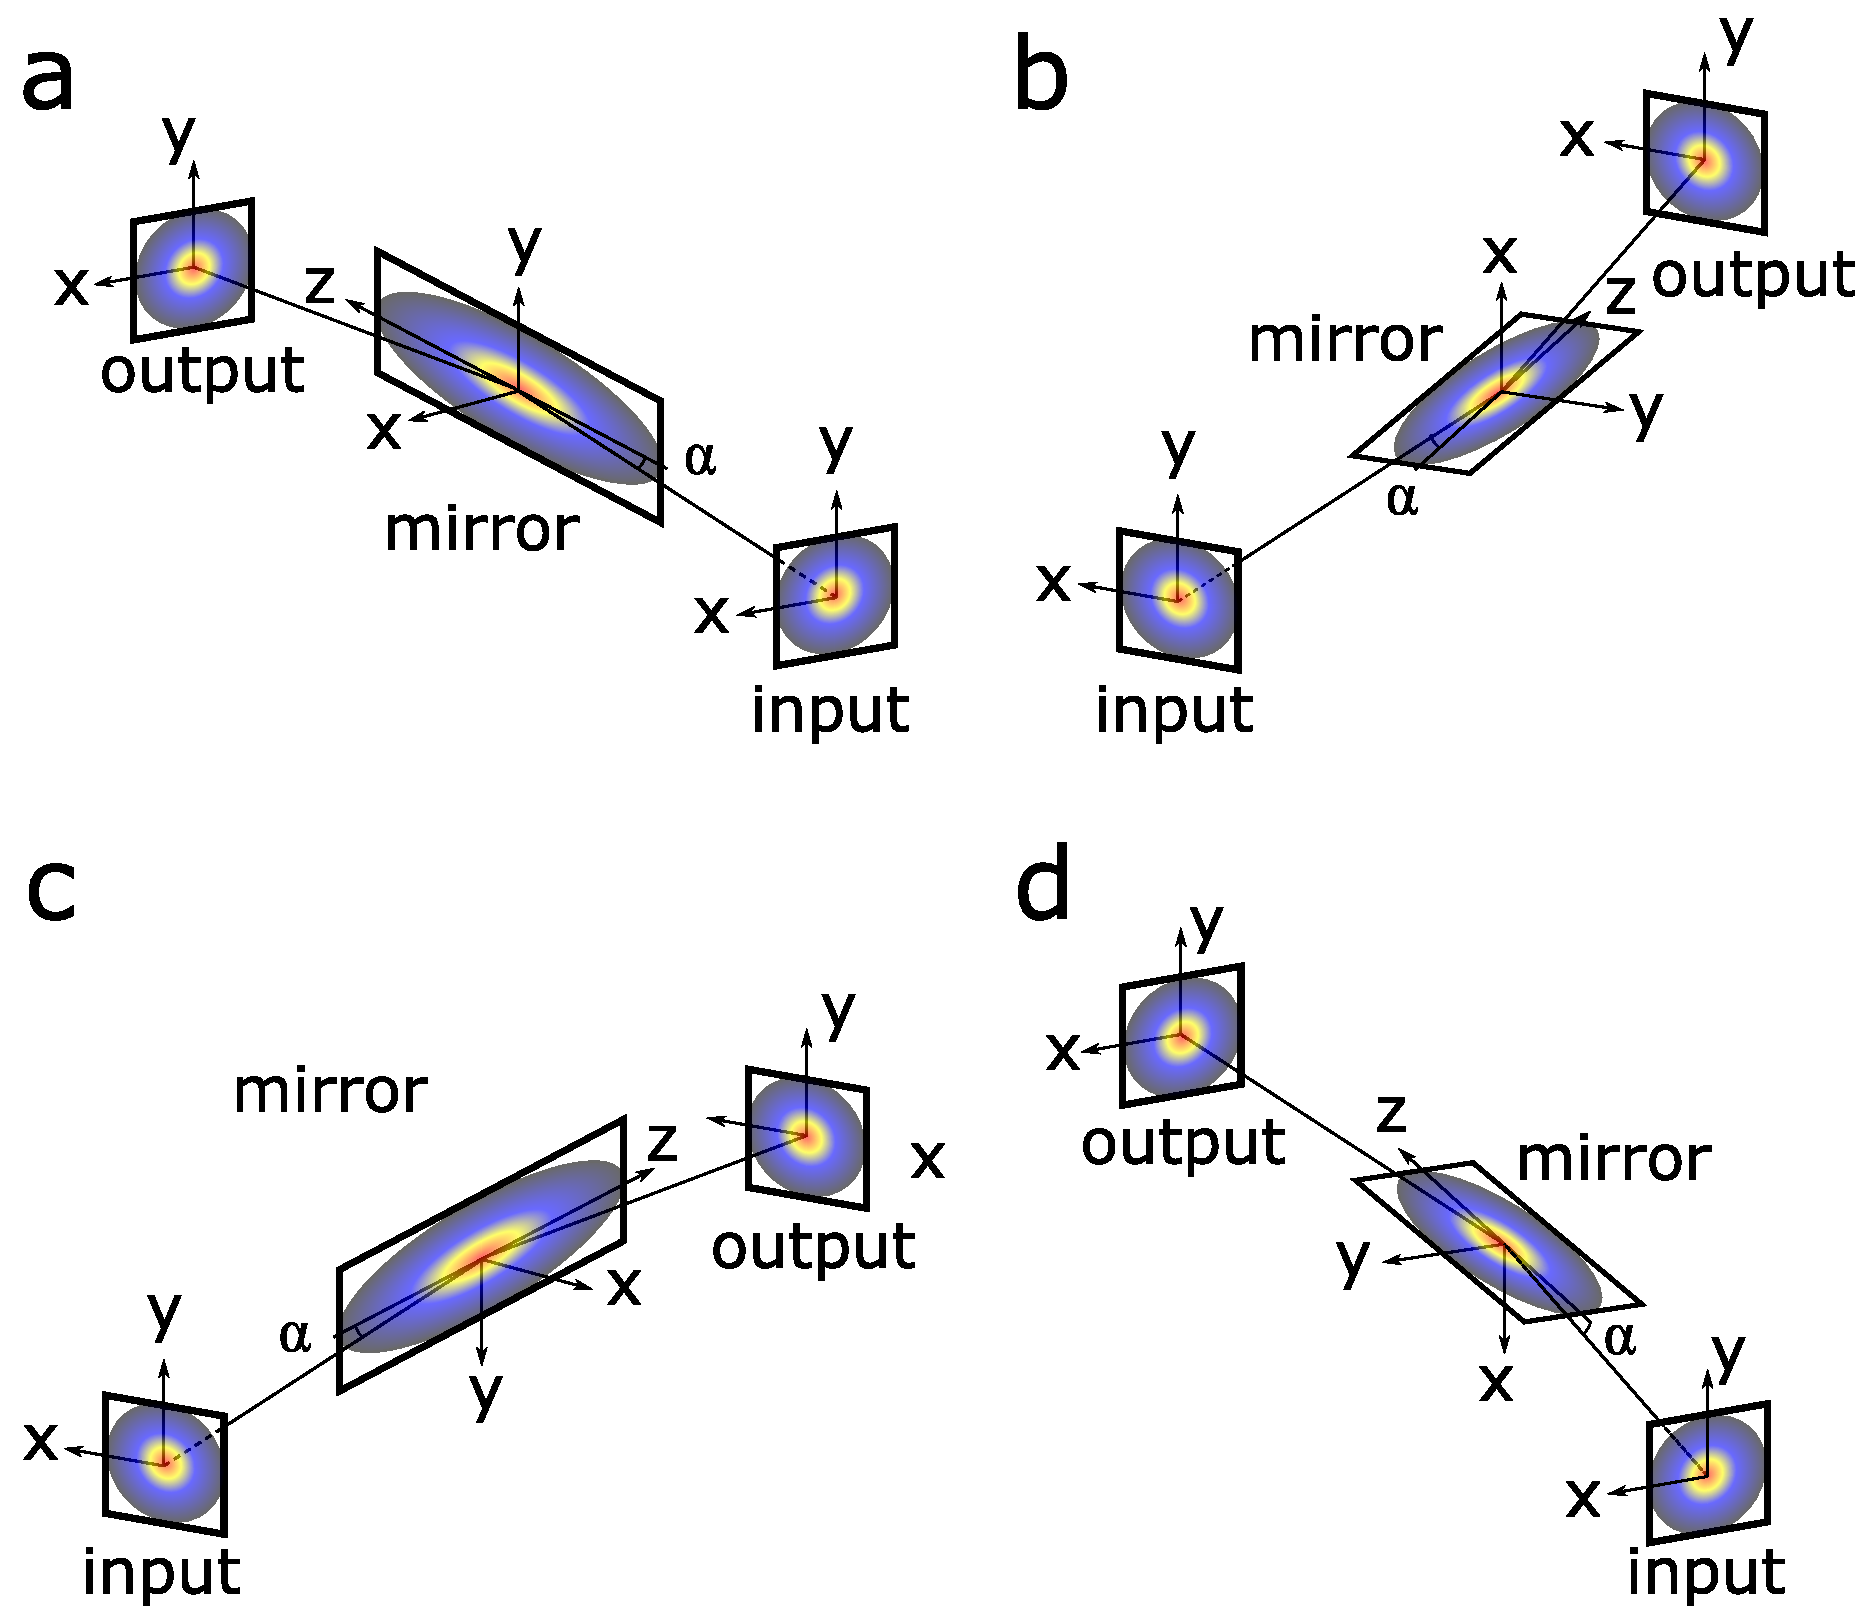
\includegraphics[width=1.0\textwidth]{Figures/coordinates.pdf}
\caption{Coordinate system definition for beam and mirror. Beam coordinates follow the LCLS convention, with the z direction pointing in the direction of propagation. For the mirror coordinates, the x-axis is always defined to be the surface normal, and the z-axis is always defined to point in the direction of propagation,  roughly parallel to the beam's z-axis. (a) $0^\circ$ orientation, with the mirror y-axis aligned with the beam's y-axis, with angle of incidence $\alpha$ (referred to as orientation ``0''). (b) $90^\circ$ orientation (y-axis is rotated $90^\circ$ about the z-axis relative to (a)), with angle of incidence $\alpha$ (orientation ``1''). (c) $180^\circ$ orientation (orientation ``2''). (d) $270^\circ$ orientation (orientation ``3''). A positive angle is defined to be a counter-clockwise rotation about a given axis. The orientation in (a) results in a deflection of the beam in the positive x-direction, and (b) results in a deflection of the beam in the positive y-direction. The orientations in (c) and (d) result in deflections in the negative x- and y-directions, respectively.}
\label{fig:coordinates}
\end{center}
\end{figure}

See Fig.~\ref{fig:mirror_motion} for reference on the effect of mirror translation relative to its normal vector. There are two main effects: the beam is centered on a different point on the mirror, and the beam is translated upon reflection in the beam's x-axis direction. As can be seen from the figure, a mirror motion $\delta x_m$ causes the beam to be shifted (in mirror coordinates) along the mirror's z-axis by
\begin{equation}
\label{delta_z}
\delta z_m = -\frac{\delta x_m}{\tan\alpha}.
\end{equation}
Secondly, the beam is translated by
\begin{equation}
\label{delta_cx}
\delta x_b = 2 \delta x_m \cos\alpha.
\end{equation}
There is also a minor effect of a change in the beam's path length. The change is simply given by $\overline{AD} - (\overline{AB} + \overline{BC})$:
\begin{equation}
\label{path_length}
%cos alpha = AD / (2 delta_z)
%cos alpha = delta_z / AB
%AD = 2 delta_z cos = 2 cos (delta_x/tan) = 2 delta_x cos^2 / sin
%AB = delta_z / cos = delta_x/(tan cos) = delta_x / sin
\delta z_b = \frac{2 \delta x_m}{\sin\alpha} \cos^2\alpha - \frac{2 \delta x_m}{\sin\alpha} = -2 \delta x_m \sin\alpha.
\end{equation}
For small adjustments $\delta x_m$ and small glancing angles this is smaller than a typical Rayleigh range, so it is safe to ignore this small change in path length.

\begin{figure}[htb]
\begin{center}
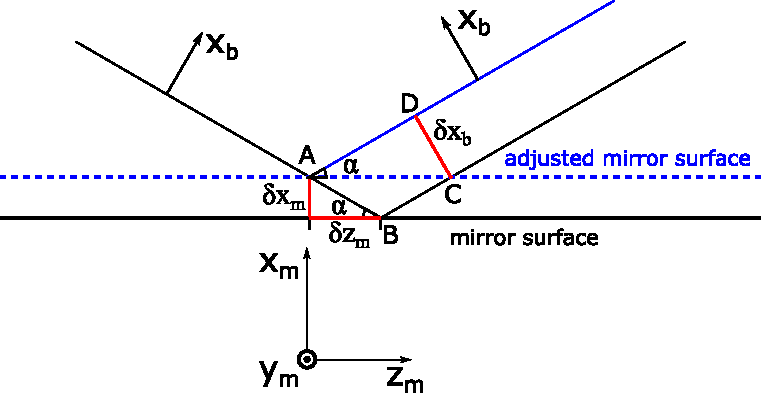
\includegraphics[width=1.0\textwidth]{Figures/mirror_motion.pdf}
\caption{Effect of mirror translation parallel to the surface normal (mirror x-axis). Note the vertices A, B, C, and D that are referenced in the text.}
\label{fig:mirror_motion}
\end{center}
\end{figure}

Another consideration is the effect of a change in the beam's center relative to the beam x-axis. See Fig.~\ref{fig:beam_shift} for reference. From the figure it is clear that for a shift in the beam's center, $\delta x_b$, the beam moves by a distance $\delta z_m$ on the mirror surface given by
\begin{equation}
\label{eq:beam_shift}
\delta z_m = \frac{\delta x_b}{\sin\alpha}.
\end{equation}
Secondly, upon reflection the beam center on the beam's x-axis changes sign, as depicted in Fig.~\ref{fig:beam_shift}.

\begin{figure}[htb]
\begin{center}
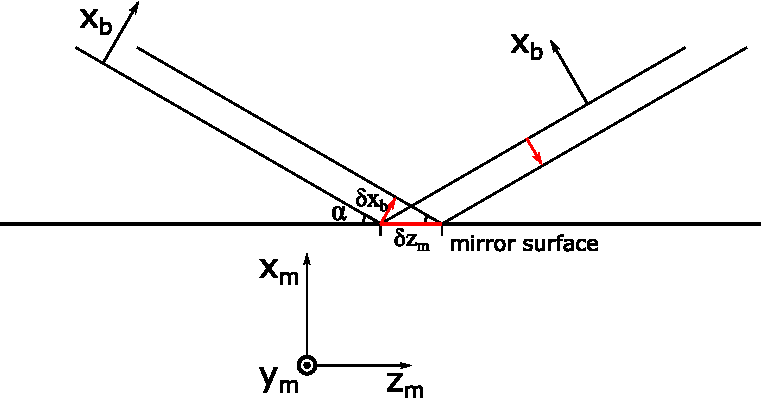
\includegraphics[width=1.0\textwidth]{Figures/beam_shift.pdf}
\caption{Effect of beam center shift in the plane of incidence.}
\label{fig:beam_shift}
\end{center}
\end{figure}

In order to account for phase errors in the reflected beam due to height errors on a surface, the change in path length due to the height error must be calculated. See Fig.~\ref{fig:phase_error} for reference. In the figure, $\alpha$ is the angle of incidence. For convenience the angle $\gamma$ is defined as
\begin{equation}
\gamma = \frac{\pi}{2} - 2 \alpha
\end{equation}
As mentioned in the caption for Fig.~\ref{fig:phase_error}, the path length difference is given by the difference in segment lengths $\overline{AB} - \overline{AC}$. The segment lengths are given by:
\begin{equation}
\label{eq:AC}
\overline{AC} = \frac{h}{\sin\alpha}
\end{equation}
\begin{equation}
\overline{AB} = \frac{h}{\sin\alpha} \sin\gamma = \frac{h}{\sin\alpha} \left( 1 - 2 \sin^2\alpha \right)
\end{equation}
The path length difference is then given by
\begin{equation}
\Delta z = \overline{AB} - \overline{AC} = - 2 h \sin\alpha
\end{equation}
with a resulting phase change of
\begin{equation}
\label{eq:mirror_phase}
\Delta \phi = - \frac{4 \pi}{\lambda} h \sin\alpha.
\end{equation}

\begin{figure}[htb]
\begin{center}
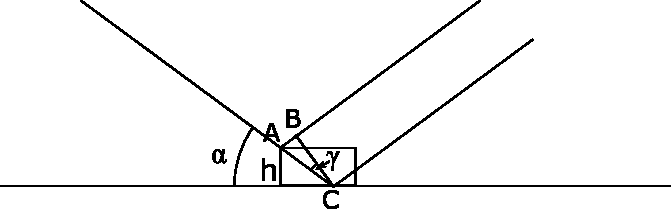
\includegraphics[width=1.0\textwidth]{Figures/phase_error.pdf}
\caption{Effect of small height error on the reflected phase. The path length difference due to height error is $\overline{AB} - \overline{AC}$.}
\label{fig:phase_error}
\end{center}
\end{figure}

An analogous expression can be found for the effects of a height error on a grating surface. The difference is that the diffracted beam exits at a different angle, leading to slight change in the path length. See Fig.~\ref{fig:grating_phase_error} for reference. The path length difference is again $\overline{AB} - \overline{AC}$. Here the angle $\gamma$ is slightly different. It is now
\begin{equation}
\gamma = \frac{\pi}{2} - \beta - \alpha
\end{equation}
The length of $\overline{AC}$ is still given by Eqn.~\ref{eq:AC}. The length of $\overline{AB}$ becomes
\begin{equation}
\overline{AB} = \overline{AC} \sin\gamma = \frac{h}{\sin\alpha} \sin\gamma
\end{equation}
This gives a path length difference of
% sin(gamma) = sin(pi/2-beta-alpha) = cos(alpha+beta)
% cos(alpha+beta) = 1 - 2 sin^2((alpha+beta)/2)
\begin{equation}
\Delta z = \overline{AB} - \overline{AC} = \frac{h}{\sin\alpha} \left(\sin\gamma - 1 \right) = \frac{-2 h}{\sin\alpha},\sin^2\left(\frac{\alpha+\beta}{2}\right)
\end{equation}
giving a phase change of
\begin{equation}
\Delta \phi = \frac{-4 \pi h}{\lambda \sin\alpha} \sin^2\left(\frac{\alpha+\beta}{2}\right)
\end{equation}
We see that when $\alpha=\beta$ as in the case of a mirror this reduces to the result obtained in Eq.~\ref{eq:mirror_phase}.



\begin{figure}[htb]
\begin{center}
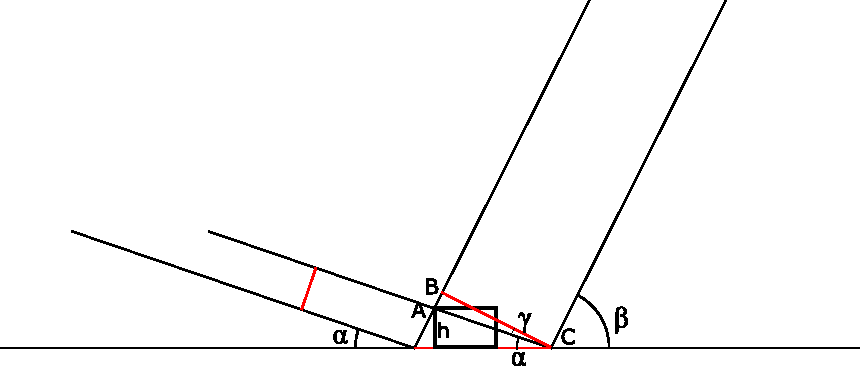
\includegraphics[width=1.0\textwidth]{Figures/grating_phase_error.pdf}
\caption{Effect of small height error on the reflected phase for a grating. The path length difference due to height error is $\overline{AB} - \overline{AC}$.}
\label{fig:grating_phase_error}
\end{center}
\end{figure}

\subsection{FlatMirror class}
\label{FlatMirror}

\subsection{CurvedMirror class}
\label{CurvedMirror}

\subsection{Grating class}

\subsection{Mono class}

\subsection{Collimator class}

\subsection{Slit class}

\subsection{Drift class}

\subsection{CRL class}

\subsection{PPM class}
PPM is facing upstream.

\section{beamline2d subpackage}

\subsection{Beamline class}\label{beamline}

\section{Future Developments}

Future developments will include
\begin{itemize}
  \item{a Pulse class in order to propagate for example SASE pulses through a beamline, and see the effect on the time structure.}
  \item{Methods to interfere two beams/pulses and view the resulting interference pattern.}
  \item{Tracking device and beam positions in absolute coordinates, along with some form of viewing this in 3D.}
  \item{Crystals for hard X-ray monochromators, including miscut feature.}
  \item{Additional mirror types such as ellipsoids.}
  \item{Better simulation of elliptical mirror including the unequally spaced mapping of beam coordinates to mirror coordinates.}
\end{itemize}

\end{document}
